\documentclass[12pt]{standalone}

% tikz
\usepackage{lmodern}                                       % solve font issue
\usepackage[T1]{fontenc}

\usepackage{tikz}
\usepackage{pgfplots}

\usepgfplotslibrary{fillbetween}                           % LaTeX and plain TeX
\pgfplotsset{width=190pt,height=190pt,compat=1.15}         % compatibility for PGFPlots 1.15

% color
\definecolor{xdxdff}{rgb}{0.49,0.49,1}
\definecolor{qqwuqq}{rgb}{0,0.39,0}

\begin{document}

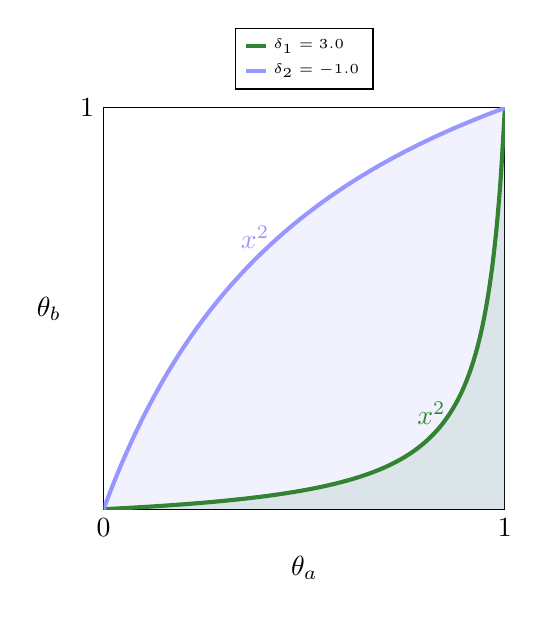
\begin{tikzpicture}
	\pgfmathsetmacro{\deltaOne}{3.0}
	\pgfmathsetmacro{\deltaTwo}{-1}
	\begin{axis} [
			xmin=0,xmax=1,xtick={1},xtick style={draw=none},
			ymin=0,ymax=1,ytick={1},ytick style={draw=none},
			extra x ticks={0},
			xlabel=$\theta_a$, ylabel=$\theta_b$, ylabel style={rotate=-90},
			axis equal=true,
			enlargelimits=false,
			legend style={at={(0.5,1.2)}, anchor=north,
					legend cell align={left}, font=\tiny,
					legend image code/.code={\draw (0,0) -- (0.05,0);},
				},
		]

		% reference paths
		\path [name path=lower] (0,0) -- (1,0);
		\path [name path=upper] (0,1) -- (1,1);

		% delta > 0
		\addplot [
			name path=deltaOne,
			line width=1.5pt,
			color=qqwuqq!80,
			smooth,samples=100,domain=0:1
		] {
			x / (exp(\deltaOne) + x * (1 - exp(\deltaOne)))
		} node[above,pos=0.5] {$x^2$};;
		\addlegendentry{$\delta_1 = \deltaOne$}

		% delta < 0
		\addplot [
			name path=deltaTwo,
			line width=1.5pt,
			color=xdxdff!80,
			smooth,samples=100,domain=0:1
		] {
			x / (exp(\deltaTwo) + x * (1 - exp(\deltaTwo)))
		} node[above,pos=0.5] {$x^2$};
		\addlegendentry{$\delta_2 = \deltaTwo$}

		\addplot [
			qqwuqq,fill opacity=0.1
		] fill between [
				of=deltaOne and lower,
			];

		\addplot [
			xdxdff,fill opacity=0.1
		] fill between [
				of=deltaTwo and lower,
			];

	\end{axis}
\end{tikzpicture}
\end{document}